\RequirePackage[l2tabu, orthodox]{nag}
\documentclass[version=last, pagesize, twoside=off, bibliography=totoc, DIV=calc, fontsize=12pt, a4paper, french, english]{scrartcl}
%Setting pdfgentounicode to one permits (together with package glyphtounicode) to copy eg x ⪰ y iff v(x) ≥ v(y) from pdf to unicode data. 
	\pdfgentounicode=1 
	\input{glyphtounicode}
%Latin Modern has more glyphs than Computer Modern, such as diacritical characters, and permits copy from resulting PDF. fntguide commands to load the font before fontenc, to prevent default loading of cmr.
	\usepackage{lmodern}
%Encode resulting accented characters correctly in resulting PDF, permits copy from PDF.
	\usepackage[T1]{fontenc}
%UTF8 seems to be the default in recent TeX installations, but not all. https://tex.stackexchange.com/a/370280
	\usepackage[utf8]{inputenc}
%Provides \newunicodechar for easy definition of supplementary UTF8 characters such as → or ≤ for use in source code.
	\usepackage{newunicodechar}
%Text Companion fonts, much used together with CM-like fonts. Provides \texteuro and other similar commands for text mode characters such as \textminus, \textrightarrow, \textlbrackdbl.
	\usepackage{textcomp}
%Solves bug in lmodern, https://tex.stackexchange.com/a/261188. (TODO see if useful?)
	%Declare `cmex` to be arbitrary scalable.
	\DeclareFontShape{OMX}{cmex}{m}{n}{
	  <-7.5> cmex7
	  <7.5-8.5> cmex8
	  <8.5-9.5> cmex9
	  <9.5-> cmex10
	}{}
	\SetSymbolFont{largesymbols}{normal}{OMX}{cmex}{m}{n}
	\SetSymbolFont{largesymbols}{bold}  {OMX}{cmex}{m}{n}
%More symbols available in bold version, see https://github.com/latex3/latex2e/issues/71.
	\DeclareFontShape{OMX}{cmex}{bx}{n}{%
	   <->sfixed*cmexb10%
	   }{}
	\SetSymbolFont{largesymbols}{bold}{OMX}{cmex}{bx}{n}
%Warn about missing characters.
	\tracinglostchars=2
%\usepackage{booktabs}
%TODO should be loaded!
%\usepackage{calc}
%\usepackage{tabularx}
%Provides \addtocmd, \patchcmd, \newtoggle commands.
	\usepackage{etoolbox} 
%mathtools requires amsmath, which is anyway considered a basic, mandatory package nowadays (Grätzer, More Math Into LaTeX).
	\usepackage{amsmath}
%Seems better to load mathtools before babel.
%mathtools fixes some bugs in amsmath; permits to hide (non manual) tags that are never referenced; provides \refeq for truthful typesetting of manual tag references and \DeclarePairedDelimiter.
	\usepackage{mathtools} 
	\mathtoolsset{showonlyrefs, showmanualtags}
%Package frenchb asks to load natbib before babel-french. Package hyperref asks to load natbib before hyperref.
	\usepackage{natbib}
%Language options ([french, english]) should be on the document level (last is main).
%TODO do not remove babel, which beamer uses (beamer uses the \translate command for the appendix); but french can be removed.
%	\usepackage{babel}
%	\frenchbsetup{AutoSpacePunctuation=false}
%\usepackage{listings}
	%\lstset{tabsize=2}
%I favor acro over acronym because the former is more recently updated (2017 VS 2015 at time of writing); has a longer user manual (about 40 pages VS 6 pages if not counting the example and implementation parts); has a command for capitalization; and acronym suffers a nasty bug when ac used in section, see http://tex.stackexchange.com/questions/103483/strange-packages-interaction-acronyms-silence-hyperref (though this might be the fault of the silence package and might be solved in more recent versions, I do not know).
	%\usepackage{acro}

\newtoggle{LCpres}
\togglefalse{LCpres}

\iftoggle{LCpres}{
	%I favor fmtcount over nth because it is loaded by datetime anyway; and fmtcount warns about possible conflicts when loaded after nth.
	\usepackage{fmtcount}
	%For nice input of date of presentation. Must be loaded after the babel package. Has possible problems with srcletter: https://golatex.de/verwendung-von-babel-und-datetime-in-scrlttr2-schlaegt-fehlt-t14779.html.
	\usepackage[nodayofweek]{datetime}
}{
}
%I do not use option pdfusetitle (which must be introduced here and not in hypersetup) in articles because the title often has some asterisk or other supplement that must not appear in the pdf metadata. For presentations, Beamer implicitely uses the pdfusetitle option.
	\usepackage{hyperref}
	%I hide links for those which can be recognized as links by the reader without highlighting, to not distract the reader. urlbordercolor is used both for \url (and \doi) and for \href, thus might need to be removed. TODO test in presentation.
	\hypersetup{linkbordercolor={1 1 1}, citebordercolor={1 1 1}, urlbordercolor={1 1 1}}
	%hyperref doc says: “Package bookmark replaces hyperref’s bookmark organization by a new algorithm (...) Therefore I recommend using this package”.
	\usepackage{bookmark}
%Need to invoke hyperref explicitly to link to line numbers: \hyperlink{lintarget:mylinelabel}{\ref*{lin:mylinelabel}}, with \ref* to disable automatic link. Also see https://tex.stackexchange.com/questions/428656/external-cross-reference-to-a-line-number-using-lineno-and-xr-hyper for referencing lines from another document.
	%\usepackage{lineno}
	%\newcommand{\llabel}[1]{\hypertarget{lintarget:#1}{}\linelabel{lin:#1}}
	%\setlength\linenumbersep{9mm}
%For complex authors blocks. Seems like authblk wants to be later than hyperref, but sooner than silence.
	\nottoggle{LCpres}{
		\usepackage{authblk}
		\renewcommand\Affilfont{\small}
	}{
	}
%I do not use floatrow, because it requires an ugly hack for proper functioning with KOMA script (see scrhack doc). Instead, the following command centers all floats, and I manually place my table captions above and figure captions below their contents (https://tex.stackexchange.com/a/3253).
	\makeatletter
	\g@addto@macro\@floatboxreset\centering
	\makeatother
%Permits to customize enumeration display and references
	%\nottoggle{LCpres}{
		%\usepackage{enumitem} %follow enumerate by a string saying how to display enumeration
	%}{
	%}
%Provides \Cen­ter­ing, \RaggedLeft, and \RaggedRight and en­vi­ron­ments Cen­ter, FlushLeft, and FlushRight, which al­low hy­phen­ation. 
	%\usepackage{ragged2e}
%To typeset units by closely following the “official” rules.
	%\usepackage[strict]{siunitx} %[expproduct=tighttimes, decimalsymbol=comma] ou (plus récent ?) [round-mode=figures, round-precision=2, scientific-notation = engineering]
%My favorites bibliographystyle’s provide doi’s. The package doi turns those into urls. However, it uses old-style dx.doi url (see 3.8 DOI system Proxy Server technical details, “Users may resolve DOI names that are structured to use the DOI system Proxy Server (http://doi.org (preferred) or http://dx.doi.org).”, https://www.doi.org/doi_handbook/3_Resolution.html). The patch solves this.
	\usepackage{doi}
	\makeatletter
	\patchcmd{\@doi}{dx.doi.org}{doi.org}{}{}
	\makeatother
%Makes sure upper case greek letters are italic as well.
	\usepackage{fixmath}
%Provides \mathbb; obsoletes latexsym (see http://tug.ctan.org/macros/latex/base/latexsym.dtx). Relatedly, \usepackage{eucal} to change the mathcal font and \usepackage[mathscr]{eucal} (apparently equivalent to \usepackage[mathscr]{euscript}) to supplement \mathcal with \mathscr. This last option is not very useful as both fonts are similar, and the intent of the authors of eucal was to provide a replacement to mathcal (see doc euscript). Also provides \mathfrak for supplementary letters.
	\usepackage{amsfonts}
%Provides a beautiful (IMHO) \mathscr and really different than \mathcal, for supplementary uppercase letters. TODO drawback is that no bold version!?
	\usepackage{mathrsfs}
%Multiple means to produce bold math: \mathbf, \boldmath (defined to be \mathversion{bold}, see fntguide), \pmb, \boldsymbol (all legacy, from LaTeX base and AMS), \bm (the most recommended one), \mathbold from package fixmath (I don’t see its advantage over \boldsymbol).
%“The \boldsymbol command is obtained preferably by using the bm package, which provides a newer, more powerful version than the one provided by the amsmath package. Generally speaking, it is ill-advised to apply \boldsymbol to more than one symbol at a time.” — AMS Short math guide. “If no bold font appears to be available for a particular symbol, \bm will use ‘poor man’s bold’” — bm. It is “best to load the package after any packages that define new symbol fonts” – bm. bm defines \boldsymbol as synonym to \bm.  \boldmath accesses the correct font if it exists; it is used by \bm when appropriate. See https://tex.stackexchange.com/a/10643 for some difficulties with \bm.
%TODO check how to make it warn when no bold or poor bold.
	\usepackage{bm}
%amsthm corrects the spacing of proclamations, allows for theoremstyle, and is considered a basic, mandatory package nowadays (Grätzer, More Math Into LaTeX).
	\usepackage{amsthm}
%Provides \cref. Unfortunately, cref fails when the language is French and referring to a label whose name contains a colon (https://tex.stackexchange.com/questions/83798/cleveref-varioref-missing-endcsname-inserted). cleveref should go “laster” than hyperref.
	\usepackage{cleveref}
%\usepackage{tikz}
	%\usetikzlibrary{babel, matrix, fit, plotmarks, calc, trees, shapes.geometric, positioning, plothandlers, arrows, shapes.multipart}
%Vizualization, on top of TikZ
	%\usepackage{pgfplots}
	%\pgfplotsset{compat=1.14}
\usepackage{graphicx}
	\graphicspath{{graphics/}}

%Provides \print­length{length}, useful for debugging.
	%\usepackage{printlen}
	%\uselengthunit{mm}
%Provides \NewDocumentCommand and similar commands intended as replacement of \newcommand in LaTeX3 (for package authors? https://tex.stackexchange.com/questions/98152/always-use-newdocumentcommand-instead-of-newcommand TODO).
	\usepackage{xparse}

\iftoggle{LCpres}{
	%“fixes the frame num­ber­ing in beamer when us­ing an ap­pendix such that the slides from the ap­pendix are not counted in the to­tal frame num­ber of the main part of the doc­u­ment”.
		\usepackage{appendixnumberbeamer}
	%I have yet to see anyone actually use these navigation symbols – this command removes them.
		\setbeamertemplate{navigation symbols}{}
	\usepackage{preamble/beamerthemeParisFrance}
}{
}
%tikzposter-specific
%remove \usepackage{ragged2e}: causes 1=1 to be printed in the middle of the poster. (Anyway prints a warning about those characters being missing.)
%put [french, english] options next to \usepackage{babel} to avoid warning

%TODO Compare $\sum$ and $\boldsymbol{\sum}$ and ${\mathversion{bold} \sum}$. Check whether nag should be loaded first (it says strange things).


\newcommand{\R}{ℝ}
\newcommand{\N}{ℕ}
\newcommand{\powerset}[1]{\mathscr{P}(#1)}%TODO \mathscr rather than \mathcal: scr is rounder than cal (at least in XITS Math).
%Powerset without zero.
\newcommand{\powersetz}[1]{\mathscr{P}*(#1)}
%Better than using the package braket because braket introduces possibly undesirable space. Then: $\set{x \in \R^2 \suchthat {|x|}<5}$.
\newcommand{\set}[1]{\left\{#1\right\}}
\newcommand{\suchthat}{\mathrel{}\middle|\mathrel{}}
%TODO test Integer interval.
\newcommand{\intvl}[1]{⟦#1⟧}
%TODO test
%\newcommand{\card}[1]{\lvert{}#1\rvert}
\DeclarePairedDelimiter\abs{\lvert}{\rvert}
\DeclarePairedDelimiter\card{\lvert}{\rvert}
\DeclarePairedDelimiter\norm{\lVert}{\rVert}
\DeclareMathOperator*{\argmax}{arg\,max}
\DeclareMathOperator*{\argmin}{arg\,min}

\AtBeginDocument{%
	\renewcommand{\epsilon}{\varepsilon}
% TODO we want straight form of \phi for mathematics, as recommended in UTR #25: Unicode support for mathematics.
	\renewcommand{\phi}{\varphi}
}

% with amssymb, but I don’t want to use amssymb just for that.
% \newcommand{\restr}[2]{{#1}_{\restriction #2}}
%\newcommand{\restr}[2]{{#1\upharpoonright}_{#2}}
%\newcommand{\restr}[2]{{#1|}_{#2}}%sometimes typed out incorrectly within \set.
%TODO test https://tex.stackexchange.com/a/278631
\newcommand\restr[2]{#1\raisebox{-.5ex}{$|$}_{#2}}
%\newcommand{\restr}[2]{{#1}_{\vert #2}}%\vert errors when used within \Set and is typed out incorrectly within \set.



%Decision Theory (MCDA and SC)
\newcommand{\allalts}{\mathscr{A}}
\newcommand{\alts}{A}
\newcommand{\dm}{d}

%Social Choice
%TODO unify cal and scr
\newcommand{\allF}{\mathcal{F}}
\newcommand{\allvoters}{\mathscr{N}}
\newcommand{\voters}{N}
%TODO bold math?
\newcommand{\profiles}{\linors^N}
\newcommand{\allprofs}{\mathcal{R}}
\newcommand{\pref}{\succ}
\newcommand{\prof}{\mathbf{R}}
\newcommand{\profdet}[1][u_i]{(#1, i \in \mathscr{N})}
\newcommand{\rprof}{\mathbf{x}}
\newcommand{\linors}{\mathcal{L}(\allalts)}
\newcommand{\weakors}[1][\allalts]{\mathcal{W}(#1)}

%Axiomatics
\newcommand{\pbasic}[1]{\prof^{#1}_\epsilon}
\newcommand{\pelem}[1]{\prof^{#1}_e}
\newcommand{\pcycl}[1]{\prof^{#1}_c}
\newcommand{\pcycllong}[1]{\prof^{#1}_{cl}}
\newcommand{\pinv}[1]{\overline{\prof_{#1}}}
\newcommand{\alllang}{\mathcal{L}}
\newcommand{\ltru}{\texttt{T}}
\newcommand{\lfal}{\texttt{F}}
\newcommand{\laxiom}[1]{\textsc{#1}}
\newcommand{\lequiv}{\Vvdash}

%Deliberated Judgement
%TODO mathrel, etc.?
\newcommand{\ileadsto}{\rightsquigarrow}
\newcommand{\mleadsto}[1][\eta]{\rightsquigarrow_{#1}}
\newcommand{\ibeats}{\vartriangleright}
\newcommand{\mbeats}[1][\eta]{\vartriangleright_{#1}}

%ARG TH
\newcommand{\AF}{\mathcal{AF}}
\newcommand{\labelling}{\mathcal{L}}
\newcommand{\labin}{\textbf{in}\xspace}
\newcommand{\labout}{\textbf{out}}
\newcommand{\labund}{\textbf{undec}\xspace}
\newcommand{\allargs}{A^*}
\newcommand{\args}{A}
\newcommand{\ar}{a}
\newcommand{\ext}{\mathcal{E}}

%MCDA
\newcommand{\allcrits}{\mathcal{C}}
\newcommand{\cat}[1]{C_{#1}}
\newcommand{\cats}{\mathcal{C}}
\newcommand{\alttoc}[2][x]{(#1 \xrightarrow{} #2)}
\newcommand{\alttocat}[3]{(#2 \xrightarrow{#1} #3)}
\newcommand{\alttoI}{(x \xrightarrow{} \left[\underline{C_x}, \overline{C_x}\right])}
\newcommand{\alttocatdm}[3][t]{\left(#2 \thinspace \raisebox{-3pt}{$\xrightarrow{#1}$}\thinspace #3\right)}
\newcommand{\alttocatatleast}[2]{\left(#1 \thinspace \raisebox{-3pt}{$\xrightarrow[]{≥}$}\thinspace #2\right)}
\newcommand{\alttocatatmost}[2]{\left(#1 \thinspace \raisebox{-3pt}{$\xrightarrow[]{≤}$}\thinspace #2\right)}


\input{preamble/redac}
\input{preamble/draw}

\begin{document}
\title{%
	\texorpdfstring{
		Visu blah%
		\thanks{
			This is a draft.
		}
	}{%
		Visu
	}
}
\author{Renaud Blanch}
\author{Sylvain Bouveret}
\affil{LIG}
\author{Olivier Cailloux}
\affil{Université Paris-Dauphine, PSL Research University, CNRS, LAMSADE, 75016 PARIS, FRANCE\\
	\href{mailto:olivier.cailloux@dauphine.fr}{olivier.cailloux@dauphine.fr}
}
\maketitle

\section{Introduction}
\label{sec:intro}
Voting rules are prominent objects used in social choice theory to aggregate preference information and obtain a societal choice.

Various rules treat the profile, the information given as input, differently, according to the transformations considered to not change the information \citep{sen_social_1986, sen_informational_1974, sen_weights_1977, blackorby_social_1984}.

\section{Profile and visual variables}
Here we indicate which information a profile contains and how this corresponds to visual variables.
We have then to relate this to visual variables.

We consider defined a set of alternatives $\allalts$ and a set of voters $\allvoters$. The preference of a voter $i \in \allvoters$ is represented by a linear order $\pref_i \subseteq \allalts × \allalts$ (a transitive, connected and antisymmetric binary relation) over the alternatives. The set of all linear orders is denoted by $\linors$, thus $\pref_i \in \linors$. A profile $\prof: \allvoters → \linors$ associates each voter to her preference. The set of all profiles is $\allprofs = \linors^\allvoters$. A voting rule $f: \allprofs → \powersetz{\allalts}$, where $\powersetz{S}$ denotes the set of all non empty subsets of $S$, associates to each profile a set of winners, a non-empty subset of the alternatives. Sets are used to tolerate ties.

\begin{figure}[t]
	\centering
	\begin{tikzpicture}
		\tikzset{prof matrix/.style={
			matrix, column sep=3mm, row sep=2mm
		}}
		\tikzset{rank-vector/.style={
			draw, rectangle, inner sep=0, outer sep=1mm
		}}
		
		\path node[prof matrix] (profile) {
			\path node {$R_1$};&
			\path node {$R_2$};
			\\
			\path node {$a$};&
			\path node {$a$};
			\\
			\path node {$b$};&
			\path node {$c$};
			\\
			\path node {$c$};&
			\path node {$b$};
			\\
		};
		\path[draw, decorate, decoration={brace, mirror}] (profile.south west) -- (profile.south east);
		\path ($(profile.south west)!.5!(profile.south east)$) ++ (0, -5mm) node {$\prof \in \linors^\allvoters$};
		
		\path (profile.north east) ++ (1.5cm, 0) node[prof matrix, anchor=north west] (rank-profile) {
			&
			\path node (header start) {1};&
			\path node (header end) {2};
			\\
			\path node (alts start) {$a$};&
			\path node (rv1 start) {1};&
			\path node (rv1 end) {1};
			\\
			\path node {$b$};&
			\path node (rv2 start) {2};&
			\path node (rv2 end) {3};
			\\
			\path node (alts end) {$c$};&
			\path node (rv3 start) {3};&
			\path node (rv3 end) {2};
			\\
		};
		\path node[draw, ellipse, dotted, inner sep=0, fit=(header start.north west) (header end.south east)] (N) {};
		\path (N.north) node[anchor=south, inner sep=1mm] {$\allvoters$};
		\path node[draw, ellipse, dotted, inner sep=0, fit=(alts start.north west) (alts end.south east)] (A) {};
		\path (A.west) node[anchor=east, inner sep=1mm] {$\allalts$};
		\path[draw, decorate, decoration={brace, mirror, raise=2mm}] (rank-profile.south west) -- (rank-profile.south east);
		\path ($(rank-profile.south west)!.5!(rank-profile.south east)$) ++ (0, -7mm) node {$\prof \in (\R^\allalts)^\allvoters$};
	\end{tikzpicture}
	\caption{Alternative ways of viewing a profile (reusing a figure by \citet{cailloux_eliciting_2014}, with permission)}
	\label{fig:rankprofile}
\end{figure}

The information contained in a profile can be viewed in various ways. For example, instead of displaying the linear orders below each voters, as is most classical, the profile may be viewed as a matrix which indicates, for each alternative and voter, the rank of the alternative in the ranking of the voter \citep{cailloux_eliciting_2014}. See \cref{fig:rankprofile}.
More generally, we view a profile as a \emph{scoring profile}, an association of numbers to voters and alternatives: each voter is associated to a utility function $u_i: \allalts → \R$, which describes the “score” this voter gives to each alternative. Thus, we denote a scoring profile by $\prof = \profdet$. (Abusing notation, we reuse the same letter $\prof$ to denote a scoring profile under this more general conception and reuse the letter $\allprofs$ to denote the set of all scoring profiles.)

In the following, we will also consider the (weighted) majority graph of a profile. The \emph{majority margin} $m$ is the function that maps each pair of candidates $(x, y) \in \allalts^2$ to the difference between the number of voters that prefer $x$ to $y$ and the number of voters that prefer $y$ to $x$, namely: $m(x, y) = |\{i\in N:\ x \pref_i y\}| - |\{i\in N:\ y \pref_i x\}|$.  The \emph{majority relation} is the binary relation $\succeq_{\Maj}$ defined as the subset of elements $(x, y) \in N^2$ such that $m(x, y) \geq 0$. The binary relation $\pref_{\Maj}$ is the strict part of $\succeq_{\Maj}$; therefore if $x \pref_{\Maj} y$, we say that $x$ (strictly) beats $y$ in a pairwise election (or comparison). The \emph{weighted majority graph} $\mathcal{WG}$ is the weighted directed graph representing $\succeq_{\Maj}$, with $m(x,y)$ being the weight of arc $(x, y)$. The majority graph $\mathcal{G}$ is the unweighted version of the weighted majority graph. A \emph{Condorcet winner} is a candidate that strictly beats every other candidate in a pairwise election, that is, the only candidate (if any) that has no incoming edge in $\mathcal{G}$.

Interestingly, depending on the purpose of the visualization, the informational content to be taken into account may change. In order to let the viewer focus on the relevant information, the informational content in the profile may be reduced. For example, if the focus is to explain the Condorcet property, it may be adequate to display only information necessary to deduce the majority graph. Or, when being interested in scoring rules, it may be desired to display only, for each alternative, the ranks it obtained, that is, a multi-set of ranks, neglecting the relation between the voters and the ranks. Conversely, in some cases, such as in the context of exemplifying a given voting rule, it may be desired to show more than the information contained in the profile. A prominent example is the one of scoring rules: when the scores to be used are known, what is to be aggregated may be viewed as the scores given by each voter to each alternative. In yet other cases, the information to be visualized is both poorer and richer (in different respects), as when showing, for each alternative, a multiset of scores with no individual link between the voters and the scores.

In this section we want to classify systematically visualization approaches depending on the informational content to be taken into account, in order to move towards being able to select an appropriate visualization in a principled way. Informational content can be characterized thanks to an equivalence relation on the set of scoring profiles $\allprofs$. 
\begin{description}
	\item[OM-NC] To start with, consider \emph{Ordinally Measurable, Noncomparable Utilities}: in this interpretation, two profiles are equivalent iff they describe the same orderings for each voter. Formally, a profile $\prof = \profdet[u_i]$ is considered equivalent to any profile $\prof' = \profdet[\phi_i(u_i)]$ where $\phi_i: \R^\allalts → \R^\allalts, i \in N$ are non-decreasing transformations of the utilities. When using this interpretation of the informational content of a profile, only the orderings represented by the utilities count. This is the classical input information considered for a voting rule, as described above.
	\item[CM-NC] One can also attribute more meaning to the numbers in the utility functions. In the \emph{Cardinally Measurable, Noncomparable Utilities} interpretation, the $\phi_i$ transformations must be of the form $\phi_i(u_i) = a_i + b_i u_i$ for some $a_i \in \R, b_i \in \R^{*+} = \R \cap (0, +\infty)$.
	\item[CM-FC] The \emph{Cardinally Measurable, Fully Comparable Utilities} interpretation mandates that the $\phi_i$ transformation be of the form $\phi_i(u_i) = a + b u_i$ for some $a \in \R, b \in \R^{*+}$, the same for all voters. In other words, it supplements the requirements of the previous interpretation by forcing equality of the transformations: $\phi_i = \phi_j \forall i, j \in \allvoters$.
	\item[PM-FC] The \emph{Proportionally Measurable, Fully Comparable Utilities} interpretation \commentOC{We should decide whether we like that name.} allows only transformations of the form $\phi_i(u_i) = b u_i$, $b \in \R^{*+}$.
	\item[WMG] In the \emph{Weighted Majority Graph} interpretation, two profiles are equivalent iff they have the same weighted majority graph.
	\item[MG] In the \emph{Majority Graph} interpretation, two profiles are equivalent iff they have the same majority graph.
	\item[RC] In the \emph{Rank Count} interpretation, two profiles are equivalent iff, for each alternative and rank, the number of times the alternative receives the rank (is positioned at that rank by some voter) is the same in both profiles.
	\item[SC] The \emph{Score Count} interpretation is similar to RC except the alternatives must receive each scores (not merely rank) the same number of times.
	\item[SS] For the \emph{Sum Scores} interpretation, the sum of the scores is what matters: two profiles are equivalent iff, for each alternative, the sum of the scores received in both profile match.
\end{description}
Other interpretations are defined by \citet{blackorby_social_1984}, from which we took some of these interpretations.

An equivalence relation $\sim$ on the set of scoring profiles is said to be finer than another equivalence relation $\sim'$ iff $\prof \sim \prof' ⇒ \prof \sim' \prof'$, thus, iff $\sim \subseteq \sim'$, or still equivalently, iff $\sim$ defines smaller equivalence classes than $\sim'$. In that case, the interpretation associated to $\sim$ is said to be richer than the interpretation associated to $\sim'$, and conversely, the latter interpretation is said to be poorer. Equivalently, an interpretation is richer than another one iff any profile transformation $\phi$ that does not cross the boundary of an equivalence class in the richer interpretation also does not cross equivalence classes in the poorer interpretation. Finally, it is still equivalent to say that an interpretation is richer than another one iff, given any equivalence class of the richer interpration, there is exactly one equivalence class of the poorer interpretation that contains all the given equivalence class.

\Cref{fig:poorer} shows the relation between some of the just defined interpretations.
\begin{figure}
	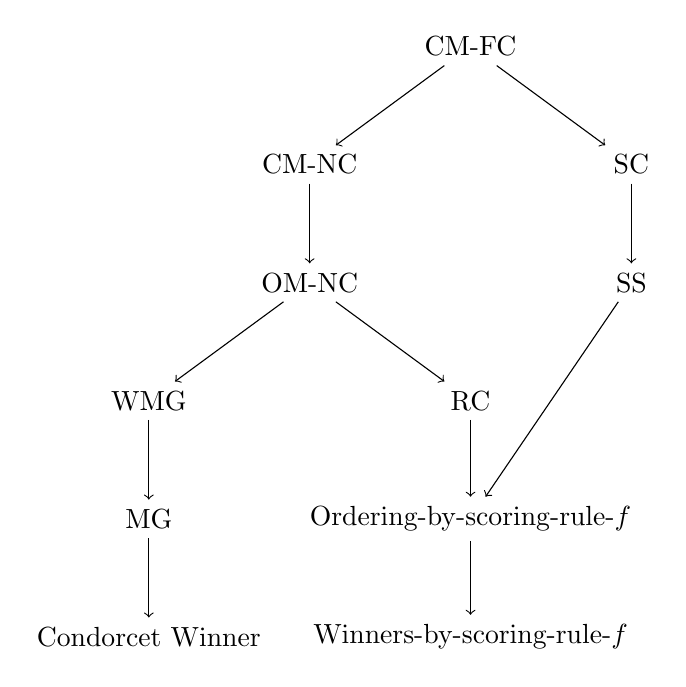
\begin{tikzpicture}
		\path[edge from parent/.style={draw, ->}, sibling distance=27ex] node {CM-FC} child {
			node {CM-NC} child {
				node {OM-NC} child {
					node {WMG} child {
                                        	node {MG} child {
                                                	node {Condorcet Winner}
                                                }
					}
				} child {
					node {RC} child {
						node (O) {Ordering-by-scoring-rule-$f$} child {
							node {Winners-by-scoring-rule-$f$}
						}
					} 
				}
			} 
		} child {
			node {SC} child {
				node (SS) {SS}
			}
		};
		\path[draw, ->] (SS) -- (O);
	\end{tikzpicture}
	\caption{A part of the richer-than relation.}
	\label{fig:poorer}
\end{figure}

One of our goals is to select appropriate visualizations given a profile $\prof$ and an interpretation $\sim$ on a (partly) principled basis. In order to do this, we must first, for each interpretation, indicate what is to be visualized in order to pay due attention to the equivalence classes defined by $\sim$. Indeed, the numbers shown in a profile, or that can be deduced from the information present in a profile, relate to each others in different ways depending on the interpretation: in some cases, only ordinal comparisons matter, in other cases, more can be drawn from these numbers. 

TODO: relate to visualization variables. Possibly, talk about how to switch from one representation to another (matrix of ranks to, say, the scores). Decide whether we should introduce other kinds of interpretations (which is probably useful only if we can think about relevant visualizations). For example, we might need the \emph{Majority} interpretation, such that two profiles are considered equivalent iff they have the same majority graph.

\subsection{Graphic variables}
Giving a (possibly interactive) graphical representation to a data set is a way to make the information it contains more graspable to laymen, provided the representation is sound.
The design of such representations is studied by the Information Visualisation community.
A key step of the \emph{InfoVis Pipeline}~\citep{Chi-Riedl-1998} which transforms data into visualisations is the \emph{visual mapping}, i.e.\ the step that encodes \emph{data attributes} with \emph{graphic variables}.
For example, if each item of a data set is a person characterized by some attributes (age, genre, size, weight, etc.), we can encode a particular item with a graphic mark, and we may choose to represent the genre by its shape (e.g.\ square for men, circle for women), the weight by the abscissa, and the size by the ordinate.
The set of graphic variables that can be used without too much interference is rather small: \citet[][chap.~II.c]{bertin-graphique} gave one of the first practical list that includes 8 variables.
This list remains relevant today, even if it has been enriched latter to account for computer screens and animations~\citep[e.g.][chap.~5]{munzner}.

A key observation made by Bertin is that all graphic variables are not equal in term of expressiveness.
Some allow to judge wether two items are identical or not (e.g.\ they share the same shape), but others allow to tell wether one is bigger than the other, and even to quantify how much bigger it is (e.g.\ the abscissa of one mark is twice the abscissa of another one).
A variable is \emph{associative} ($\equiv$) if it allows to represent different levels without inducing a visual hierarchy between those levels.
A variable is \emph{selective} ($\neq$) if all items sharing a level (e.g.\ same color) can be perceived as a group and considered for inspection without the items of other levels interfering.
A variable is \emph{ordered} ($O$) if we can order two items according to this variable, without relying on a lookup to a legend.
Finally, a variable is \emph{quantitative} ($Q$) if we can quantify the difference between two items.

The two cartesian dimensions (when working in the plane) of the \emph{position} are two variables that are the most expressive: they support $\equiv$, $\neq$, $O$ and $Q$.
The \emph{size} of the mark is also very expressive: it supports $\neq$, $O$ and $Q$ but not $\equiv$ (large marks will pop up).
The \emph{value}, i.e.\ the grey level independently of the hue, is also $\neq$ and $O$ but not $\equiv$ and not $Q$ (darker grey will pop up on a white background and we can not quantify how much darker or lighter is a grey from another grey).
The \emph{texture} (the scale of a given pattern used to fill a mark) is $\equiv$, $\neq$ and $O$, but not $Q$.
The \emph{color}, i.e.\ the hue independently of the grey level, is both $\equiv$ and $\neq$, but can not be used for $O$ and $Q$.
The \emph{orientation} can be used for $\equiv$ and, to a certain extend, for $\neq$, provided the shape of the mark does not present too much symmetries.
Finally, the \emph{shape} of the mark can be used only for $\equiv$ if the various shapes are carefully chosen.

\subsection{Relating informational content and visual variables}
Depending on the task that the visualisation is used for, different kind and richness of information should be presented. For example, if the task is to find a Condorcet winner given a profile, it seems adequate to choose a visualisation which allows to clearly see the majority graph (an information somewhat poorer than the rank profile, in the sense that the information class is wider). If the task is to find the Borda winners given a profile, the visualisation could on the contrary enrich the rank profile by giving access to the scores, and it should do so by encouraging the user to perform quantitative comparisons (Q) rather than just permit ordinal comparisons as is adequate with ranks information or majority-graph information.

Given a scoring profile $\prof$ and an interpretation under the form of an equivalence relation $\sim$ on the set of profiles, we can define which information should be visible in a visualization of $\prof$ under $\sim$. To check that this summarized information is appropriate, we can check that any two equivalent profiles (according to $\sim$) have the same summarized information (in which case the summary contains no more than allowed); and that any two non equivalent profiles have different visualization (in which case the summary contains no less than allowed). 
 Note that this does not guarantee absence of redundant information.
We write $O$ to refer to an ordering, $I$ to indicate an information of interval scale type, and $A$ for absolute, where no transformation of the numbers is allowed. For example, under the OM-NC interpretation, it should be possible to determine, for each voter, the ordering of the alternatives, which we write as an ordering over the scores.
\begin{description}
	\item[CM-FC] $a, v, s→I$ (Interval scale)
	\item[OM-NC] $a, v, s→O$
	\item[MG] $a, a, w→A$ with $w$ (for “win”) the number of victories of $a$ against $b$ (the set of tuples to display may be restricted in various ways) OR other representation as illustrated in \cref{sec:grib}, how does this classify?
	\item[RC] $a, r→O, c→A$ with $r$ the rank (in $\intvl{1, m}$), and $c$ (for “count”) the number of times this alt has received that rank OR other representation where it is explicit that the counts sum to a constant for every alternative, how does this classify? Perhaps $a, r→O, c→P$ with $P$ a proportion (in $[0, 1]$ and summing to one for a given alternative)
	\item[SS] $a, ss→Q$
	\item[SC] $a, s→Q, c→P$
\end{description}

\section{From equivalence relations to visualization}
Here we describe how we go (as automatically as possible) from the descriptions given so far to visualizations such as those illustrated in \cref{sec:grib}.

\section{Tasks and visualization}
We wish to illustrate the usefulness of this classification on two kinds of tasks. 

\subsection{Train to identify winners}
The first kind of task is: train the user to compute some kind of winners by himself, given a profile viewed in a given way. This is done in two phases. First, in the training phase, the user is shown a profile, using some (possibly several) visualizations, to help him understand what is expected from him and how the winner is computed. Second, in the test phase, the user is shown only the profile with the imposed visualization, and has to find the winner by himself.

For this kind of task, we expect it will be helpful to the user to see the profile with varying informational content (varying interpretations). For example, for computing the Condorcet winner, it might be helpful in the training phase to see the starting profile, the profile reduced to its majority graph information, and the resulting Condorcet winner. For computing the Borda winners, it might be helpful, starting from the profile considered as linear orders, to train the user by showing the profile enriched with the score information per voter, then go to the score per alternative view, and finally show the Borda winners.

Generally, given a voting rule $f$, we search for an interpretation $\sim$, as poor as possible, that conserves the information useful to $f$: such that $f(\prof) = f(\prof')$ if $\prof \sim \prof'$. (This information is generally known in the literature from axiomatic analysis, or obvious, for most well-known voting rules.) In general, for voting rules (working on ordinal profiles), we search an interpretation poorer than or equal to OM-NC, with the exception of scoring rules. 

The second kind of task is a comparison task.  Here we wish to illustrate visually the difference of “reasoning” of two voting rules. Using a principle similar to the one described above, we would search for an interpretation $\sim$ corresponding to the poorest equivalence relation (among our set of proposals described above) that conserves the information useful to $f$, and $\sim'$ corresponding to $f'$. Define $\sim^*$ the least upper bound of $\sim$ and $\sim'$, thus, the poorest equivalence relation that is richer than both $\sim$ and $\sim'$. Then we show, to illustrate $f$ and $f'$ on $\prof$, the interpretation of $\prof$ using $\sim^*$, then on one side of the screen, $\sim$ and the winners according to $f$; on the other side of the screen, $\sim'$ and the winners according to $f'$.

Or something like that.

\bibliography{Visu,manual}
\appendix
\section{Gribouilling}
\label{sec:grib}
Let’s see what we gribouilled, to help us with the task of categorization.

\begin{figure}
	\includegraphics[trim={400 300 150 700}, clip, width=\textwidth, height=9cm, keepaspectratio]{Gribouillis1.jpeg}
	\caption{Gribouillis1}
	\label{fig:g1}
\end{figure}

\Cref{fig:g1}, from top left, by line. $r$: rank, $v$: voter, $a$: alternative, $n$: nb times; $L$: line width, $SX$: sub-x, $C$: color, $XI\alpha$: x interval (varying interval size with minimal size=$\alpha$, $\alpha \in \{0, 1\}$), $T$: texture
\begin{enumerate}
	\item $v→X, a→Y, r→SYI0$
	\item $v→X, a→Y, r→SXI0$
	\item $v→X, a→Y, r→L$
	\item $v→X, r→Y, a→C$
	\item $voters / aggregation→X, v→SX, a→Y, r→SSX[X=left], n→SXI0[X=right], r→SY$
	\item $n→XI1, r→T, a→Y$ (hence, visible that the sum is constant)
	\item $v→X, a→Y, r→T$
	\item $v→X, a→Y, r→SX$
	\item $r→X, a→Y, n→SXI1, n→SYI1$
\end{enumerate}

\begin{figure}
	\includegraphics[trim={0 200 0 600}, clip, width=\textwidth, height=9cm, keepaspectratio]{Gribouillis2.jpeg}
	\caption{Gribouillis2}
	\label{fig:g2}
\end{figure}
\Cref{fig:g2}.
\begin{description}
	\item[middle left] several sub-views with animations for transitions to next sub-view.
	\begin{enumerate}
		\item $a→X, v→Y, r→SX, r→SY$.
		\item $Y$ indicates the majority relation [using cycle reduction], $X$ used to distinguish alternatives in the same majority cycle, and inside each zone, a vector shows ranks with $[v→SX, r→SSX, r→SSY]$. 
		\item maj. rel. → Y, a→(x, y), v→SX, preference direction→arrow direction. 
		\item same with pairs of arrows in opposite directions being striken (remaining arrows indicate who wins each pairwise battle).
	\end{enumerate}
	\item[bottom left] $votes/counts/sums→X, v→SX[X=left], a→Y, r→SSX[X=left], r→SY[X=left], n→SXI[X=center], r→SY[X=center], n→SXI[X=right], r→SYI[X=right]$ (change $Y$ interval size depending on score corresponding to the rank number, on example: half for second place, zero for third place). Then score is total resulting area. NB the center and right parts are not totally separate.
	\item[top right] from rank-count (displayed horizontally), show scores (as 2D shapes) after transformation using a score function.
	\item[middle] v→X, r→Y, a→C, r→SXI, r→SYI
\end{description}

\section{Another possible starting point}
We call \emph{snapshot} a particular piece of information to be shown to the user \commentOC{TODO find a better name}. Let us distinguish snapshots by kind, depending on the operations permitted.
\begin{itemize}
	\item A snapshot $s$ of kind “Orders per voter”, $s \in \weakors^\allvoters$, corresponds to the usual conception of a profile: it associates each voter to a weak order on the set of alternatives. \commentOC{I switched to weak orders, to be discussed.}
	\item The kind “Intensities per voter”, $s = (s_1, s_2), s_1 \in \weakors^\allvoters, s_2 \in \weakors[\allalts × \allalts]^\allvoters$ permits, in supplement, for each voter, to compare differences of preference between two alternatives, for example, voter $i$ has a bigger difference of preference for $a$ compared to $b$ than for $c$ compared to $d$.
	\item The kind “Comparable intensities”, $s = (s_1, s_2), s_1 \in \weakors^\allvoters, s_2 \subseteq (\allvoters × \allalts × \allalts)$ permits, in supplement, to compare differences of preferences across voters, for example, voter $i$’s difference of preference for $a$ compared to $b$ is bigger than voter $j$’s difference of preference for $c$ compared to $d$.
	\item The kind “Scores per voter”, $s \in (\R^\allalts)^\allvoters$ associates each voter and alternative to an absolute score given by that voter to this alternative. It permits to compare intensities across voters, and…  (to be continued?)
	\item The kind “Enumerate orders”, $s \subseteq \weakors$, only permits to enumerate weak orders, but not to know which voter each is associated to.
	\item The kind “Majorities strengths”, $s \in \intvl{1, n}^(\allalts × \allalts)$, permits to associate to each pair of alternatives the number of persons who strictly prefer the first one to the second one.
\end{itemize}

\section{Properties of visu}
We consider a visualization of a profile under an interpretation as a function $V_\sim(\prof)$ that maps profiles to drawings, $V: \allprofs → D$, with $D$ the set of possible drawings (we do not describe $D$). We consider it is possible to apply a renaming to the resulting drawing and that it is an internal operation, thus, for any $V$, we consider defined, for any permutation $\sigma$ on $\allalts$, an internal operation $\sigma_D: V(\allprofs) → V(\allprofs)$, where $V(\allprofs) \subseteq D$ is the image of $V$.

When the visualization should show a profile $\prof$ under an interpretation $\sim$, the visualization should satisfy the following properties.
\begin{description}
	\item[neutrality] The visualization treats all alternatives equally: if $\prof'$ contains the same information with alternatives renamed using a permutation $\sigma$ on $\allalts$, then $V(\prof') = \sigma(V(\prof))$.
\end{description}

\section{Representative elements}
This is probably too complex wrt the added value (if any).

We define for each interpretation a set containing exactly one element per equivalence class in $\sim$. Thus some mapping, which we leave implicit, maps any two profiles $\prof, \prof'$ in the same equivalence class to the same element of the set (there is an injection from $\allprofs/\sim$ to the set). We also indicate which operations are meaningful in the given interpretation, using the following notation. $D(E)$ represents the set $E$ together with a simple discrimination operation, meaning that the elements of $E$ can be distinguished, but no other operation is allowed. $W(E)$ represents the set of weak-orders on the set $E$, and indicates that, in supplement to distinguishing the elements, the elements of $E$ can be compared pairwize to determine which one is greater. $A(\succeq)$, for some weak-order $\succeq$ over some $E$, represents $(\R^+ ∪ \{\infty\})^\succ$, with $\succ$ the strict part of $\succeq$, and allows to determine, in supplement to an ordering over $E$, how many times an element of $E$ is greater than another (smaller) element of $E$. $I(E)$ represents $\set{(\succeq, f) \suchthat \succeq \in W(E), f \in A(\succeq^*) \text{ for some } \succeq^* \in W(\succ)}$: it allows, in supplement to $W(E)$, to determine how many times a difference between a pair of elements of $E$ is greater than another difference between a pair of elements of $E$, thus, it is an interval scale.
\begin{description}
	\item[CM-FC] $I(\allalts × \allvoters)$.
	\item[CM-NC] $I(\allalts)^{D(\allvoters)}$. Example with one voter and utility function: $(a, 9), (b, 5), (c, 4)$. Then $\succ = \{(a, b), (b, c), (a, c)\}$, $\succeq^* = \{((a, c), (a, b)),\allowbreak ((a, b), (b, c)),\allowbreak ((a, c), (b, c)),\allowbreak ((a, b), (a, b)),\allowbreak ((b, c), (b, c)), ((a, c), (a, c))\}$, $A(\succeq^*) = (\R^+ ∪ \{\infty\})^{\succ^*}$, and $f = \{((a, c), (a, b), 5/4), ((a, b), (b, c), 4), ((a, c), (b, c), 5)\}$.
	\item[OM-FC] $W(\allalts × \allvoters)$.
	\item[OM-NC] $W(\allalts)^{D(\allvoters)}$, or equivalently, $W(\allalts × \allvoters)$ but restricted to the first $m$ ranks; or can be interpreted as cardinal scores (like CM-NC) but with some restrictions on the scores.
	\item[MG] $\set{Abs(\succ) \suchthat \succ \in WS(\allalts)}$
	\item[RC] …
	\item[SS]
	\item[SC]
\end{description}

\end{document}

